\documentclass{article}
\usepackage{spconf,amsmath,epsfig}
\usepackage{tikz}
\usepackage{euscript}
\usepackage{amsfonts}
\usepackage{amssymb}
\usetikzlibrary{calc}

\newcommand{\sgn}{\operatorname{sign}}
\newcommand{\vect}{\overrightarrow}
\newcommand{\conjugate}{\overline}
\newcommand{\re}{\operatorname{Re}}
\newcommand{\im}{\operatorname{Im}}

\title{DISTORTION MEASURE OF WATERMARKING 2D VECTOR MAPS IN THE MESH-SPECTRAL DOMAIN}
\name{A. Davydov, A. Kovalev}
\address{SPb SU ITMO}

\begin{document}
%\ninept
%
\maketitle
%
\begin{abstract}
Two main claims for digital watermarking algorithms for 2D vector data are robustness against attacks and minimization of original data distortion. 
This paper proposes conformal energy as measure of original data distortion to formalize the second claim. The most satisfied the first claim among known to authors watermarking algorithms is modified 
to minimize proposed distortion measure. It can be assumed that input and output data of the watermarking algorithm is planar graph without loss of generality. 
Carried out experiments show that modified algorithm is no less resilient against random noise than original and changes angles between corresponding adjacent edges of the input and output graphs less.
\end{abstract}
%
\begin{keywords}
Laplacian, Dirichlet energy, conformal map, quadratic form, Delaunay triangulation
\end{keywords}
%
\section{Introduction}
\label{sec:intro}
2D-vector data are typically used in Geographical Information System (GIS) related applications. For its high material value due to high efforts and costs in the acquisition of the point coordinates, 
GIS-data are sometimes watermarked to protect the copyrights and customers’ registration information~\cite{Voight} or to authenticate the original GIS-data. In some special cases such as military map watermarking, 
the precise point coordinates of the restored data are highly desired compared with its original version.  

Research on digital watermarking has focused mainly on multimedia data, the research on vector data remaining relatively insufficient. 
Digital watermarking algorithms regarding vector data can be divided roughly into two categories. The first category is about spatial domain method. This methods are more studied \cite{Voight, Kim, Chang, Bazin}, 
because it allows easily to control distortion. Unfortunately, the algorithms from the first category aren't resistant enough against such attacks as random noise or inserting/deleting vertices.
Another category of algorithms of watermarking is about frequency domain method. These algorithms \cite{Ohbuchi, Ohbuchi3D, Praun} are robust against attacks, 
but on the other hand it is hard to estimate aroused distortion of the original data.
 
Another classification criterion for watermarking algorithms is using the original data during watermark extracting. Some watermarking algorithms need the original document to extract the watermark, 
they are called well-informed algorithms. By opposition, those which don’t need the original document to extract the watermark are called blind.
Blindness is an interesting property in case of huge and on the fly production of different documents as it doesn't oblige the producer to store every original document, 
but on the other hand it reduces a possibility of watermark extracting.

The most robust against different attacks (global affine transformation, object order scrambling, vertex insertion or deletion, additive random noise, cropping) algorithm among known to authors 
was proposed by Ohbuchi and others in~\cite{Ohbuchi}. It is well-informed ``frequency-domain'' algorithm, its main idea is to apply techniques developed for 3D polygonal mesh~\cite{Ohbuchi3D} to 2D-vector map. 
Hereinafter this algorithm is referred as the base algorithm. It's described briefly in section~\ref{sec:base}. Solving in this paper problem is to develop quantative measure of the original map distortion, 
our proposal is presented in section~\ref{sec:dist_measure}. We then describe the results of evaluation experiments in section~\ref{sec:results}, 
followed by a conclusion and future work in section~\ref{sec:conclusion}.

\section{Base algorithm}
\label{sec:base}
Concerned algorithm embeds message bits into a 2D vector digital map by modifying a ``frequency'' domain representation of the map. 
To compute the ``frequency'' domain representation, the algorithm first establishes connectivity among vertices of the map by using Delaunay triangulation, creating a 2D mesh that covers every vertex in the map.
The mesh is then transformed into a frequency domain representation using mesh spectral analysis proposed by Karny and others~\cite{Karni1, Karni2}. Modification of the frequency domain coefficients 
according to the message bits embeds a watermark. Inverse transforming the modified coefficient back into the coordinate domain produces a map with the watermark embedded. The modification of coefficients in the
frequency domain ultimately displaces vertex coordinates in the spatial domain.

For computational efficiency and for robustness against cropping, a map is first divided into many rectangular subareas. Aforementioned mesh spectral analysis and watermark embedding is performed 
for each of the subareas. By embedding the same watermark repeatedly in multiple subareas, the watermark becomes resilient against cropping.

Watermarks are extracted by comparing the \textit{reference map} (the map before watermarking) with the watermarked and possibly attacked \textit{watermark map}. The two maps are first geometrically registered by
using an iterative optimization process to minimize distance among a set of landmarks. This registration could remove an affine transformation applied to the watermarked map. Then the area subdivision 
equal to the one used for the embedding is recreated on the reference map, and the subdivision is transferred to the watermarked map. For each corresponding subarea, mesh spectral analysis and then comparison of
spectral coefficients recovers the embedded watermark.

Let's consider the process of watermark embedding in detail. Let $V = \{v_1, v_2, \dots, v_n\}$ is set of vertices of the reference map, $n = |V|$. Let $\mathfrak{T}$ denote some triangulation of the set $V$, 
$G(\mathfrak{T})$ denote graph of the triangulation $\mathfrak{T}$. The eigenvectors $\{\mathbf{e}_i\}_{i=1}^n$ of the graph $G(\mathfrak{T})$ are the eigenvectors of its Laplacian. 
There are several different Laplacian matrices, for example \cite{Biggs, Chung, Zhang}. Bigg's definition of Laplacian $R$ is employed in the base algorithm
$$R = I - D^{-1} A,$$ where $I$ is the identity matrix, $D$ is a diagonal matrix whose diagonal element $D_{ii} = deg(v_i)$ is inverse degree of the vertex $i$ of the graph $G(\mathfrak{T})$. 
$A$ is the adjacency matrix of the graph $G(\mathfrak{T})$
\begin{eqnarray*}
  D_{ij} = \begin{cases} deg(v_i) &\text{if $i = j$,} \\ 0 &\text{otherwise;} \end{cases} \\
  A_{ij} = \begin{cases} 1 &\text{if vertices $i$ and $j$ is adjacent,} \\ 0 &\text{otherwise.} \end{cases} 
\end{eqnarray*}
The eigenvectors $\{\mathbf{e}_i\}_{i=1}^n$ constitute basis of $\mathbb{R}^n$. We can assume that eigenvectors are normalized, $||e_i|| = 1$. 
Let $v_i = (x_i, y_i)$ then $\mathbf{r} = (r_1, r_2, \dots, r_n)$, $\mathbf{s} = (s_1, s_2, \dots, s_n)$ are decompositions of the vectors $\mathbf{x} = (x_1, x_2, \dots, x_n)^T$, 
$\mathbf{y} = (y_1, y_2, \dots, y_n)^T$ correspondingly in the basis $\{\mathbf{e}_i\}_{i=1}^n$. In the other words 
\begin{eqnarray*}
  \mathbf{x} = r_1 \mathbf{e}_1 + r_2 \mathbf{e}_2 + \dots + r_n \mathbf{e_n}; \\ 
  \mathbf{y} = s_1 \mathbf{e}_1 + s_2 \mathbf{e}_2 + \dots + s_n \mathbf{e_n}.  
\end{eqnarray*}
If the vectors $\{\mathbf{e}_i\}_{i=1}^n$ are orthogonal then $r_i = (\mathbf{x}, \mathbf{e}_i)$, $s_i~=~(\mathbf{y}, \mathbf{e}_i)$, but it is wrong in general case. 

Let embedded message $\mathbf{m} = (m_1, m_2, \dots, m_k)$ consists of $k$ bits, where $k \le n$, $m_i \in \{0, 1\}$. Let $q_i = 2 * m_i - 1$, $q_i \in \{-1, 1\}$.
Then change coefficients $r_i, s_i$, $1 \le k \le n$ in the following way
\begin{eqnarray*}
  r_i' = r_i + \alpha p_i q_i; \\
  s_i' = s_i + \alpha p_i q_i, 
\end{eqnarray*}
where the $\{p_i\}$ is pseudo-random number sequence generated from a private key, $\alpha$ is some positive constant. Incrementing~$\alpha$ increments resilience against attacks of the watermark, 
but simultaneously increments distortion of the reference map. And vice versa decrementing $\alpha$ decrements resilience against attacks and decrements distortion of the reference map.

Let $\mathbf{x'}, \mathbf{y'}$ are coordinates of the vertices of the watermarked map. 
\begin{eqnarray*}
  \mathbf{x'} - \mathbf{x} = (r_1' - r_1) \mathbf{e}_1 + (r_2' - r_2) \mathbf{e}_2 + \dots + (r_n' - r_n) \mathbf{e_n} = \\
  = \alpha \left[ p_1 q_1 \mathbf{e}_1 + p_2 q_2 \mathbf{e}_2 + \dots + p_k q_k \mathbf{e}_k \right], \\
  \mathbf{y'} - \mathbf{y} = \alpha \left[ p_1 q_1 \mathbf{e}_1 + p_2 q_2 \mathbf{e}_2 + \dots + p_k q_k \mathbf{e}_k \right]. 
\end{eqnarray*}
On the other words it's possible to express embedding of watermarking as constructing vector 
\begin{equation}
\label{formula:g}
 \mathbf{g} = \alpha \left[ p_1 \mathbf{w}_1 + p_2 \mathbf{w}_2 + \dots + p_k \mathbf{w}_k \right]; 
\end{equation}
$$ \mathbf{w_i} = \left( (e_{i, 1}, e_{i, 1}), (e_{i, 2}, e_{i, 2}), \dots, (e_{i, n}, e_{i, n}) \right) \mbox{ for } 1 \le i \le n. $$
If the vectors $\{\mathbf{e}_i\}_{i=1}^n$ are orthogonal and $|\mathbf{e}_i| = \frac{\sqrt{2}}{2}$ then it is possible to estimate mean length of displacement of an vertex $\Delta v_{mean}$.
\begin{equation}
\label{formula:mean_displacement}
|\mathbf{g}| = \alpha * \sqrt {k}; \mbox{      } \Delta v_{mean} = \alpha * \frac{\sqrt{k}}{n}. 
\end{equation}

To extract watermark from the watermarked map decompose vectors $\mathbf{x'} - \mathbf{x}$, $\mathbf{y'} - \mathbf{y}$ in the basis $\{\mathbf{e}_i\}_{i=1}^k$, or calculate coefficients 
$\mathbf{u} = (u_1, u_2, \dots, u_k)$, $\mathbf{w} = (w_1, w_2, \dots, w_k)$, 
\begin{eqnarray*}
  \mathbf{x'} - \mathbf{x} = u_1 \mathbf{e}_1 + u_2 \mathbf{e}_2 + \dots + u_k \mathbf{e_k}; \\ 
  \mathbf{y'} - \mathbf{y} = w_1 \mathbf{e}_1 + w_2 \mathbf{e}_2 + \dots + w_k \mathbf{e_k}.  
\end{eqnarray*}
Then bits of the embedded message can be obtained in the following way
$$q_i = \sgn(p_i * (u_i + w_i), m_i = (q_i + 1) / 2.$$

\section{Measure of distortion} 
\label{sec:dist_measure}
\subsection{Continuous case}
\label{sec:continuous}
We suppose that distortion of the refernce map is defined by the change of the angles. Let's consider some domain $\Omega \subset \mathbb{R}^2$ and function $f: \Omega \to \mathbb{R}^2$, 
$f = \begin{pmatrix} f_x(x, y) \\ f_y(x, y) \end{pmatrix}$. We assume that $f_x, f_y$ have partial derivatives with respect to $x$ and $y$. In the sequel we will use following designations:
$$
  \nabla f_x = \begin{pmatrix} \frac{\partial f_x}{\partial x} \\ \frac{\partial f_x}{\partial y} \end{pmatrix}, 
  \nabla f_y = \begin{pmatrix} \frac{\partial f_y}{\partial x} \\ \frac{\partial f_y}{\partial x} \end{pmatrix}, 
  \nabla f = \begin{pmatrix} 
    \frac{\partial f_x}{\partial x} & \frac{\partial f_x}{\partial y} \\
    \frac{\partial f_y}{\partial x} & \frac{\partial f_y}{\partial y} \\
  \end{pmatrix}. 
$$
Let's estimate change of an local angle after applying function $f$. Let $\vect{r}~=~\begin{pmatrix} x \\ y \end{pmatrix}$ is an arbitrary point, $\vect{r_1}$ is the point displaced relative to $\vect{r}$ by an arbitrary 
small vector $\vect{dr}$, 
\begin{figure}[htb]
  \begin{minipage}[b]{1.0\linewidth}
    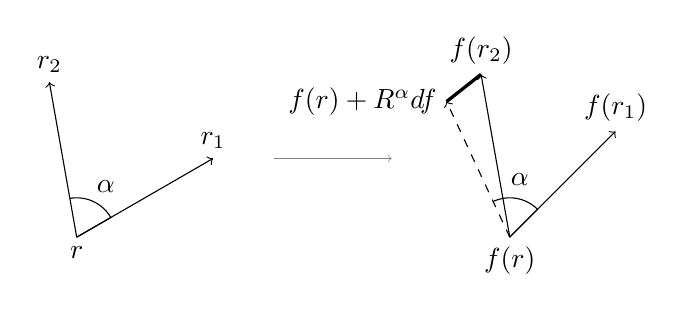
\begin{tikzpicture} 
  \coordinate[label=below:$r$]        (origin)      at (0, 0);
  \coordinate[label=above:$r_1$]   (dxdy)        at origin + (30:2);
  \coordinate[label=above:$r_2$]  (dxdyrot)     at origin + (100:2);

  \draw[->] (origin)--(dxdy);
  \draw[->] (origin)--(dxdyrot);

  \draw (origin) -- (30:0.5) arc (30:100:0.5);
  \draw (60:0.74) node {$\alpha$};
  
  \draw [help lines][ ->] (2.5, 1) -- (4.0, 1);

  \begin{scope}[shift={(0:5.5cm)}]
    \coordinate[label=below:$f(r)$]       (forigin)      at (0, 0);
    \coordinate[label=above:$f(r_1)$]  (fdxdy)        at ($(forigin) + (45:1.9)$);
    \coordinate[label=above:$f(r_2)$] (fdxdyrot)     at ($(forigin) + (100:2.1)$);
    \coordinate[label=left:$f(r) + R^\alpha df$] (rotfdxdy)    at ($(forigin) + (115:1.9)$);

    \draw[->] (forigin)--(fdxdy);
    \draw[->] (forigin)--(fdxdyrot);
    \draw[->][dashed] (forigin)--(rotfdxdy);
    \draw[very thick] (rotfdxdy)--(fdxdyrot);
    \draw (forigin) -- (45:0.5) arc (45:115:0.5);
    \draw (80:0.74) node {$\alpha$};
  \end{scope}
  %\draw (60:0.74) node {$\alpha$};
  %\draw (forigin) -- (30:0.5) arc (30:100:0.5);
  %\draw (60:0.74) node {$\alpha$};
    \end{tikzpicture} 
  \end{minipage}
  
  \caption{Change of local angle.}
  \label{fig:local_angles}
\end{figure}
$$\vect{r_1} = \vect{r} + \vect{dr} = \begin{pmatrix} x + dx \\ y + dy \end{pmatrix}$$
and $\vec{r_2}$ is the point equaled to $\vec{r_1}$ rotated relative to $\vec{r}$ by an arbitrary angle $\alpha$,
$$\vect{r_2} = \vect{r} + R^\alpha \vect{dr} = \begin{pmatrix} x \\ y \end{pmatrix} + \begin{pmatrix} \cos \alpha & -\sin \alpha \\ \sin \alpha & \cos \alpha \end{pmatrix} \begin{pmatrix} dx \\ dy \end{pmatrix},$$
where $R^\alpha$ is the rotation by angle $\alpha$ (fig. \ref{fig:local_angles}). This points are mapped to 
\begin{multline*}
  \vect{f(r)}, 
  \vect{f(r_1)} = \vect{f(r + dr)} = \vect{f(r)} + \vect{df} \approx \vect{f(r)} + (\nabla f) \vect{dr}, \\
  \vect{f(r_2)} = \vect{f(r + R^\alpha dr)} ~\approx \vect{f(r)} + (\nabla f)(R^\alpha \vect{dr}).
\end{multline*}
If $f$ preserves local angles then $f(r_2)$ must be equal to the point $f(r_1)$ rotated relative to the point~$f(r)$ by the angle $\alpha$. Otherwise we can employ length of the vector $\vect{q(r, dr, \alpha)}$
$$\vect{q(r, dr, \alpha)} = \left(\vect{f(r)} + R^\alpha \vect{df}\right) - \vect{f(r_2)}$$ as measure of the angle change.
\begin{multline}
\label{formula:angle_change_vec}
  \vect{q(r, dr, \alpha)} = \left(f(r) + R^\alpha df\right) - f(r_2) \approx \\
  \approx (f(r) + R^\alpha (\nabla f) dr) - (f(r) + (\nabla f)(R^\alpha dr)) = \\ 
  \left[R^\alpha (\nabla f) - (\nabla f) R^\alpha \right] dr. 
\end{multline}
\begin{multline}
\label{formula:ugly_commutant}
  R^\alpha (\nabla f) - (\nabla f) R^\alpha =\
  \begin{pmatrix} 
    \cos \alpha & -\sin \alpha \\ 
    \sin \alpha & \cos \alpha 
  \end{pmatrix} 
  \begin{pmatrix} 
    \frac{\partial f_x}{\partial x} & \frac{\partial f_x}{\partial y} \\
    \frac{\partial f_y}{\partial x} & \frac{\partial f_y}{\partial y} 
  \end{pmatrix} - \\
  - \begin{pmatrix} 
    \frac{\partial f_x}{\partial x} & \frac{\partial f_x}{\partial y} \\
    \frac{\partial f_y}{\partial x} & \frac{\partial f_y}{\partial y} 
  \end{pmatrix}
  \begin{pmatrix} 
    \cos \alpha & -\sin \alpha \\
    \sin \alpha & \cos \alpha 
  \end{pmatrix} = \\
  = \begin{pmatrix}
    \frac{\partial f_x}{\partial x} \cos \alpha - \frac{\partial f_y}{\partial x} \sin \alpha &
    \frac{\partial f_x}{\partial y} \cos \alpha - \frac{\partial f_y}{\partial y} \sin \alpha \\
    \frac{\partial f_x}{\partial x} \sin \alpha + \frac{\partial f_y}{\partial x} \cos \alpha &
    \frac{\partial f_x}{\partial y} \sin \alpha + \frac{\partial f_y}{\partial y} \cos \alpha 
  \end{pmatrix} - \\
  - \begin{pmatrix} 
    \frac{\partial f_x}{\partial x} \cos \alpha + \frac{\partial f_x}{\partial y} \sin \alpha &
    - \frac{\partial f_x}{\partial x} \sin \alpha + \frac{\partial f_x}{\partial y} \cos \alpha \\
    \frac{\partial f_y}{\partial x} \cos \alpha + \frac{\partial f_y}{\partial y} \sin \alpha &
    - \frac{\partial f_y}{\partial x} \sin \alpha + \frac{\partial f_y}{\partial y} \cos \alpha 
  \end{pmatrix} = \\
  = \sin \alpha \begin{pmatrix}
    -(\frac{\partial f_x}{\partial y} + \frac{\partial f_y}{\partial x}) &
    \frac{\partial f_x}{\partial x} - \frac{\partial f_y}{\partial y} \\
    \frac{\partial f_x}{\partial x} - \frac{\partial f_y}{\partial y} &
    \frac{\partial f_x}{\partial y} + \frac{\partial f_y}{\partial x} 
  \end{pmatrix}.
\end{multline}
Substituting (\ref{formula:ugly_commutant}) to the formula (\ref{formula:angle_change_vec}) obtain following formula
\begin{multline*} 
  \left| \vect{q(r, dr, \alpha)} \right| = \left| \left[R^\alpha (\nabla f) - (\nabla f) R^\alpha \right] dr \right| = \\
  = \left| \sin \alpha \begin{pmatrix}
    -(\frac{\partial f_x}{\partial y} + \frac{\partial f_y}{\partial x}) &
    \frac{\partial f_x}{\partial x} - \frac{\partial f_y}{\partial y} \\
    \frac{\partial f_x}{\partial x} - \frac{\partial f_y}{\partial y} &
    \frac{\partial f_x}{\partial y} + \frac{\partial f_y}{\partial x} 
  \end{pmatrix} dr \right| = \\
  = |\sin \alpha| \sqrt{\left(\frac{\partial f_x}{\partial y} + \frac{\partial f_y}{\partial x}\right)^2 + \left(\frac{\partial f_x}{\partial x} - \frac{\partial f_y}{\partial y}\right)^2} \left| dr \right|.
\end{multline*}
We can see that the vector $\vect{q(r, dr, \alpha)}$ vanishes when 
$$\begin{cases}
  \frac{\partial f_x}{\partial x} = \frac{\partial f_y}{\partial y} \\
  \frac{\partial f_x}{\partial y} = -\frac{\partial f_y}{\partial x} 
\end{cases}$$
i.e. $f_x$ and $f_y$ satisfy Cauchy-Riemann equations and the function $f$ is conformal. If $f$ is not conformal then length of the vector $\vect{q(r, dr, \alpha)}$ is maximal when $\alpha = \pm \frac{\pi}{2}$ 
and doesn't depend on direction of $\vect{dr}$. 
\begin{equation*}
  \left(\frac{\left| {q(r, dr, \pm \frac{\pi}{2})} \right|}{|dr|}\right)^2 = 
  \left(\frac{\partial f_x}{\partial y} + \frac{\partial f_y}{\partial x}\right)^2 + \left(\frac{\partial f_x}{\partial x} - \frac{\partial f_y}{\partial y}\right)^2 
\end{equation*}
I propose to use the functional 
\begin{equation*}
  E_C(f) = \frac{1}{2} \int_{\Omega}\left[{\left(\frac{\partial f_x}{\partial x} - \frac{\partial f_y}{\partial y}\right)^2 + \left(\frac{\partial f_x}{\partial y} + \frac{\partial f_y}{\partial x}\right)^2}\right] d\Omega   
\end{equation*}
called \textit{conformal energy} (\cite{Polthier}) as measure of distortion of the domain $\Omega$ after applying to it function $f$.

\subsection{Discrete case}
\label{sec:discrete}
Let's consider sets $V = \left\{v_1, v_2, ... , v_n\right\}$, $V' = \left\{v_1', v_2', ... , v_n'\right\}$, $v_i, v_i' \in \mathbb{R}^2$, $|V| = |V'| = n$. Let function $f: V \to V'$ maps set $V$ to set $V'$, 
$f(v_i) = v_i'$ for $1 \le i \le n$. Let $\Omega$ denote convex hull of the set $V$. We can construct Piecewise Linear Interpolation Surface (PLIS) of function values $\left\{f(v_i)\right\}_{i=1}^n$ 
using some triangulation $\mathfrak{T}$ of the set $V$, consequently $f$ can be viewed as function from $\Omega$ to~$\mathbb{R}^2$. If point $v$ is in triangle $\triangle T = (v_i v_j v_k)$, $\triangle T \in \mathfrak{T}$; 
$v = \alpha v_i + \beta v_j + \gamma v_k$, $0 \le \alpha, \beta, \gamma \le 1$, $\alpha + \beta + \gamma = 1$, then $f(v) = \alpha f(v_i) + \beta f(v_j) + \gamma f(v_k)$.
\begin{multline}
\label{formula:EC}
  E_C(f) =
  \frac{1}{2} \int_{\Omega}\left[{\left(\frac{\partial f_x}{\partial x} - \frac{\partial f_y}{\partial y}\right)^2 + \left(\frac{\partial f_x}{\partial y} + \frac{\partial f_y}{\partial x}\right)^2}\right] d\Omega = \\
  = \frac{1}{2} \int_{\Omega}\left[\left(\frac{\partial f_x}{\partial x}\right)^2 + \left(\frac{\partial f_y}{\partial y}\right)^2 + \left(\frac{\partial f_x}{\partial y}\right)^2 + 
  \left(\frac{\partial f_y}{\partial x}\right)^2 \right] d\Omega - \\
  - \int_{\Omega}\left[\frac{\partial f_x}{\partial x} \frac{\partial f_y}{\partial y} - \frac{\partial f_x}{\partial y} \frac{\partial f_y}{\partial x}\right] d\Omega = \\
  = \frac{1}{2} \int_{\Omega} \left[ \left| \nabla f_x \right| ^ 2 + \left| \nabla f_y \right| ^ 2 \right] d\Omega - \int_{\Omega} \det {\begin{pmatrix} 
    \frac{\partial f_x}{\partial x} & \frac{\partial f_x}{\partial y} \\
    \frac{\partial f_y}{\partial x} & \frac{\partial f_y}{\partial y} \\
  \end{pmatrix}} d\Omega = \\
  = E_D(f) - \int_{\Omega} \det (\nabla f) d\Omega,
\end{multline}
where $E_D(f)$ is \textit{Dirichlet energy}. It is well-known \cite{Pinkall93} that if $f$ is PLIS of function values $\left\{f_i = f(v_i)\right\}_{i=1}^n$ over triangulation $\mathfrak{T}$, then  
\begin{multline}
\label{formula:Pinkall}
  E_D(f) = \frac{1}{4} \sum_{\triangle (i, j, k) \in \mathfrak{T}} \cot{\alpha_{ij}}|f_i - f_j|^2 + \\
  + \cot{\alpha_{jk}}|f_j - f_k|^2 + \cot{\alpha_{ki}}|f_k - f_i|^2,
\end{multline}
where $\alpha_{ij}$ is the angle opposite the edge $(v_i, v_j)$ in the triangle $\triangle T = (v_i, v_j, v_k)$. The formula~(\ref{formula:Pinkall}) is equivalent to the following:
\begin{equation}
\label{formula:EDOverEdges}
  E_D(f) = \frac{1}{4} \sum_{\left( i, j \right) \in E\left(\mathfrak{T}\right)}{w_{ij} |f_i - f_j|^2}, 
\end{equation}
where $E(\mathfrak{T})$ is the edges of $\mathfrak{T}$, $w_{ij}~=~\cot\alpha_{ij}~+~\cot\alpha_{ji}$, $\alpha_{\left\{{ij, ji}\right\}}$ are the angles opposite 
to the edge~$v_i v_j$ in adjacent triangles $\triangle T_1=v_i v_j v_{k_1}$, $\triangle T_2~=~v_j v_i v_{k_2}$. If the edge~$v_i v_j$ is contained in only triangle $\triangle T=v_i v_j v_k$ 
($v_i v_j$ is contained in the bound of $\Omega$) then $w_{ij} = \cot \alpha_{ij}$.

If we assume that $f$ is complex-valued function and 
$$f_x=\re{f}=\frac{1}{2}\left(f + \conjugate{f}\right), f_y=\im{f}=\frac{1}{2}\left(f - \conjugate{f}\right),$$ 
then $$|f_i - f_j|^2 = \conjugate{(f_i - f_j)}(f_i - f_j) = (\conjugate{f_i} - \conjugate{f_j})(f_i - f_j).$$ 

Let $G(\mathfrak{T})$ denote weighted graph of the triangulation $\mathfrak{T}$, $V(G) = V$, $E(G) = E(\mathfrak{T})$, $weight(u, v) = w_{uv}$. If we consider Laplacian $L$ of the graph $G$ defined as follows 
$$L_{uv} = \begin{cases}
  \sum_{(v, x) \in E(G)}{w_{vx}}&\text{if $u = v,$} \\
  -w_{uv}&\text{if $u \sim v,$} \\
  0 &\text{otherwise;}
\end{cases}
$$ then the formula~(\ref{formula:EDOverEdges}) is equivalent to the following:
\begin{equation}
\label{formula:EDOverLaplacian}
E_D(f) = \frac{1}{4} \mathbf{f}^T L \mathbf{f},
\end{equation}
where $\mathbf{f} = (f_1, f_2, \dots f_n)^T$, $\conjugate{\mathbf{f}} = (\conjugate{f_1}, \conjugate{f_2}, \dots, \conjugate{f_n})^T$.

$\int_{\Omega} \det(\nabla f) d\Omega$ also can be viewed as value of some quadratic form applied to $\mathbf{f}$. Let's consider $\triangle T = v_i v_j v_k~\in~\mathfrak{T}$. $f$ is linear on $\triangle T$, consequently 
$\det (\nabla f)$ is constant, hence $\int_{\triangle T} \det (\nabla f) dT$ is oriented area of $\triangle T' = f_i f_j f_k$. Let's suppose that $v_i$, $v_j$, $v_k$ constitute left turn then
\begin{multline}
\label{formula:det}
  \int_{\triangle T} \det (\nabla f) dT = \frac{1}{2} (f_i - f_k) \times (f_j - f_k) = \\
  = \frac{1}{2} \left[(f_i - f_k)_x (f_j - f_k)_y - (f_i - f_k)_y (f_j - f_k)_y \right] = \\
  = \frac{i}{4} \left[ (f_i - f_k)\conjugate{(f_j - f_k)} - (f_j - f_k) \conjugate{(f_i - f_k)} \right] = \\
  = \frac{i}{4} \left[ (f_i \conjugate{f_j} - \conjugate{f_i} f_j) + (f_j \conjugate{f_k} - \conjugate{f_j} f_k) + (f_k \conjugate{f_i} - \conjugate{f_k} f_i) \right].  
\end{multline}
Substituting (\ref{formula:det}) to the formula
\begin{equation}
\label{formula:det_global}
  \int_{\Omega} \det {\left( \nabla f \right) } d\Omega = \sum_{\triangle T \in \mathfrak{T}}{ \int_{\triangle T} \det{ \left(\nabla f \right) } dT},
\end{equation}
we notice that for every edge $v_i v_j$ not contained in the bound of $\Omega$ there is the twin edge $v_j v_i$ and so expression $(f_i \conjugate{f_j}~-~\conjugate{f_i} f_j)$ is contained in the right side of 
the equation (\ref{formula:det_global}) together with the opposite expression $(f_j \conjugate{f_i} - \conjugate{f_j} f_i)$. Consequently formula (\ref{formula:det_global}) can be rewritten as
\begin{equation}
\label{formula:det_over_edges}
  \int_{\Omega} \det {\left( \nabla f \right) } d\Omega = \frac{i}{4} \sum_{v_i v_j \in \partial E}{(f_i \conjugate{f_j} - \conjugate{f_i} f_j)},
\end{equation}
where $\partial E = \partial \Omega \cap E(\mathfrak{T})$ is set of the edges of the triangulation $\mathfrak{T}$ contained in the bound of $\Omega$. If we consider matrix $L'$ defined as follows 
\begin{equation*}
  L_{uv}' = \begin{cases}
    i & \text{if edge $uv \in \partial E$ and $\Omega$ is left of the line $(u, v)$;} \\ 
    -i & \text{if edge $uv \in \partial E$ and $\Omega$ is right of the line $(u, v)$;} \\ 
    0 & \text{otherwise}
  \end{cases}
\end{equation*}
then formula~(\ref{formula:det_over_edges}) is equivalent to the following:
\begin{equation}
\label{formula:DetOverLaplacian}
  \int_{\Omega} \det {\left( \nabla f \right) } d\Omega = \frac{1}{4} \conjugate{\mathbf{f}} L' \mathbf{f}.
\end{equation}
Using formulas (\ref{formula:EC}), (\ref{formula:EDOverLaplacian}), (\ref{formula:DetOverLaplacian}) we can express $E_C(f)$ as value of some quadratic form applied to $\mathbf{f}$
\begin{equation*}
  E_C(f) = \frac{1}{4}\conjugate{\mathbf{f}} L'' \mathbf{f},
\end{equation*}
where $L'' = L - L'$. It is easy to see that $L''$ is Hermitian, consequently eigenvalues of $L''$ are real and nonnegative and eigenvectors of $L''$ are orthogonal.
If $$\mathbf{f} = \alpha \left[ p_1 + \mathbf{e}_1 + p_2 \mathbf{e}_2 + \dots + p_k \mathbf{e}_k \right],$$ where $\alpha$ is some real positive constant, $p_i \in \left\{-1, 1 \right\}$ 
and $\{\mathbf{e}_i\}_{i=1}^k$ is system of orthonormal vectors, then $E_C(f)$ will be minimized when $\{\mathbf{e}_i\}_{i=1}^k$ are the eigenvectors of $L''$ corresponding to $k$ lowest eigenvalues. 

The watermark embedding algorithm described in the section \ref{sec:base} constructs vector $\mathbf{g}$ of differences between old and new coordinates of the vertices (formula (\ref{formula:g})) and $E_C$ is functional 
applicable to $f$, $f(v) = v + g(v)$. But $$E_C(g) = E_C(f - v) = E_C(f) - E_C(v) = E_C(f),$$ because $E_C$ is linear and the identity function $v$ is conformal. 

Thereby, if one wants to use algorithm described in the section \ref{sec:base} and to minimize the distortion measure defined as conformal energy, it's necessary to select the vectors $\{\mathbf{w}_i\}_{i=1}^k$ 
from formula (\ref{formula:g}) as the eigenvectors of $L''$ corresponding to the lowest eigenvalues where $L''$ is described above.

In the section \ref{sec:continuous} we establish that $E_C(f)$ is the measure of the change of local angles. Let's consider what $E_C(f)$ expresses in the sense of the angles of the triangulation $\mathfrak{T}$ 
\begin{multline*}
  E_C(f) = E_D(f) - \int_{\Omega} \det (\nabla f) d\Omega = \\ = \frac{1}{4} \sum_{v_i v_j v_k \in \mathfrak{T}} \cot{\alpha_{ij}}|f_i - f_j|^2 + \cot{\alpha_{jk}}|f_j - f_k|^2 + \\
  + \cot{\alpha_{ki}}|f_k - f_i|^2 - 4S(f_i f_j f_k),
\end{multline*}
where $S(f_i f_j f_k)$ is oriented area of the triangule $\triangle f_i f_j f_k$. If we assume that the function $f$ distorts domain $\Omega$ a slightly, then orientation of $\triangle f_i f_j f_k$ is equal to 
the orientation of $\triangle v_i v_j v_k$ and so $\triangle f_i f_j f_k$ is oriented counterclockwise,
\begin{multline*}
  4 S(f_i f_j f_k) = \cot{\alpha_{ij}'}|f_i - f_j|^2 + \\
  + \cot{\alpha_{jk}'}|f_j - f_k|^2 + \cot{\alpha_{ki}'}|f_k - f_i|^2,
\end{multline*}
where $\alpha_{ij}'$, $\alpha_{jk}'$, $\alpha_{ki}'$ are the angles opposite to the edges $f_i f_j$, $f_j f_k$, $f_k f_i$ correspondingly. Ans so under certain assumptions
\begin{multline*}
  E_C(f) = \frac{1}{4} \sum_{v_i v_j v_k \in \mathfrak{T}} (\cot{\alpha_{ij}} - \cot{\alpha_{ij}'})|f_i - f_j|^2 + \\
  + (\cot{\alpha_{jk}} - \cot{\alpha_{jk}'})|f_j - f_k|^2 + (\cot{\alpha_{ki}} - \cot{\alpha_{ki}'})|f_k - f_i|^2.
\end{multline*}

Up to this point we have assumed that the triangulation $\mathfrak{T}$ is an arbitrary, but it is obvious that $E_C$ depends on $\mathfrak{T}$. We employ the triangulation $\mathfrak{T}$ for passing 
from discrete function values to continuous function, consequently we have to select the triangulation which minimize the roughness of a PLIS. According to theorem of Rippa \cite{Rippa, Chen} 
it is the Delaunay triangulation.  

\section{Experiment results}
\label{sec:results}
The base and modified algorithm have been tested on the two maps. The first reference map is map of rivers, it consists of polylines, 44482~vertices, 88548~edges. When magnitude $\alpha = 0.5$m, 
the watermark is 19 bits, it is embedded into 64 regions separately and duplicated 4 times, mean displacement of an vertex is 0.03m according to formula~(\ref{formula:mean_displacement}). This watermark can be restored
after applying to map additive white noise with magnitude 1.5m. Mean change of an angle between adjacent edges after applying the base algorithm is $0.64^\circ$ and after applying the proposed algorithm is $0.57^\circ$.

The second reference map is map of buildings of Saint~Petersburg, it consists of polygons, 386257~vertices. When magnitude $\alpha = 0.1$m, the watermark is 119 bits, it is embedded into 1024 regions separately 
and duplicated 3 times, mean displacement of an vertex is 0.01m. This watermark can be restored after applying to map additive white noise with magnitude 1.5m. 
Mean change of an angle after applying the base algorithm is $1.72^\circ$ and after applying the proposed algorithm is $0.97^\circ$.  

\section{Conclusion}
\label{sec:conclusion}
In this paper we presented measure of the original data distortion aroused by embedding watermark. We proposed employ conformal energy because minimization of this functional implies 
minimization of reference map angles change. Proposed measure was applied for modification of the known watermarking algorithm \cite{Ohbuchi}. Modified algorithm is equivalent to the base algorithm in the sense of 
resilience against random noise attack and changes angles less.

Our future work includes improvement of the distortion measure to take into account distortion of topology of the reference map, what can be happened in the case of intersection edges of the watermarked map.

\bibliographystyle{IEEEbib}
\bibliography{main}

\end{document}
